\documentclass[a4paper]{article}

\usepackage[english]{babel}
\usepackage[utf8x]{inputenc}
\usepackage{graphicx}
\usepackage{wrapfig}
\usepackage{lipsum}

\title{Package Example: wrapfig}
\author{writeLaTeX}

\begin{document}
\maketitle

\begin{wrapfigure}{R}{0.3\textwidth}
\centering
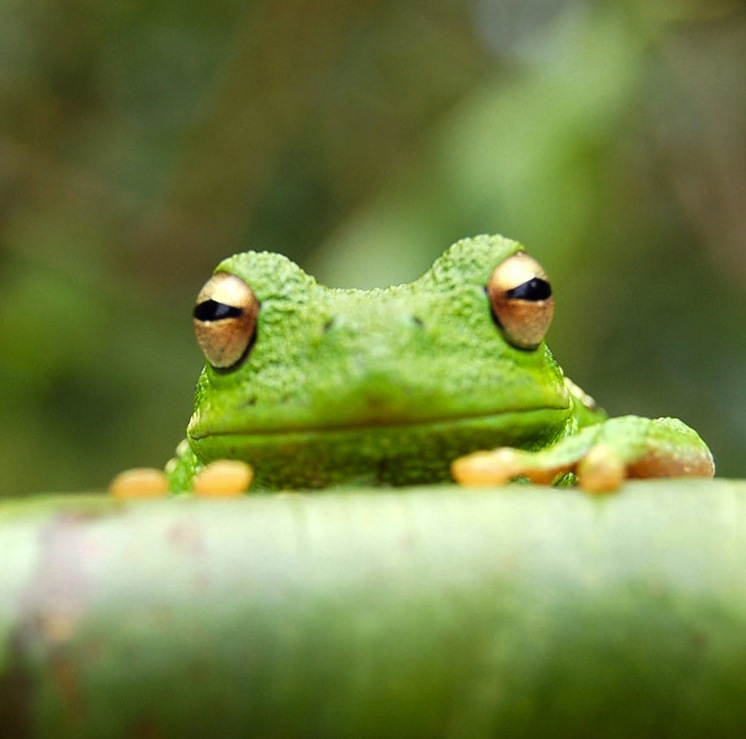
\includegraphics[width=0.25\textwidth]{frog.jpg}
\caption{\label{fig:frog1}This is a figure caption.}
\end{wrapfigure}

\lipsum[1]

\begin{wrapfigure}{L}{0.3\textwidth}
\centering
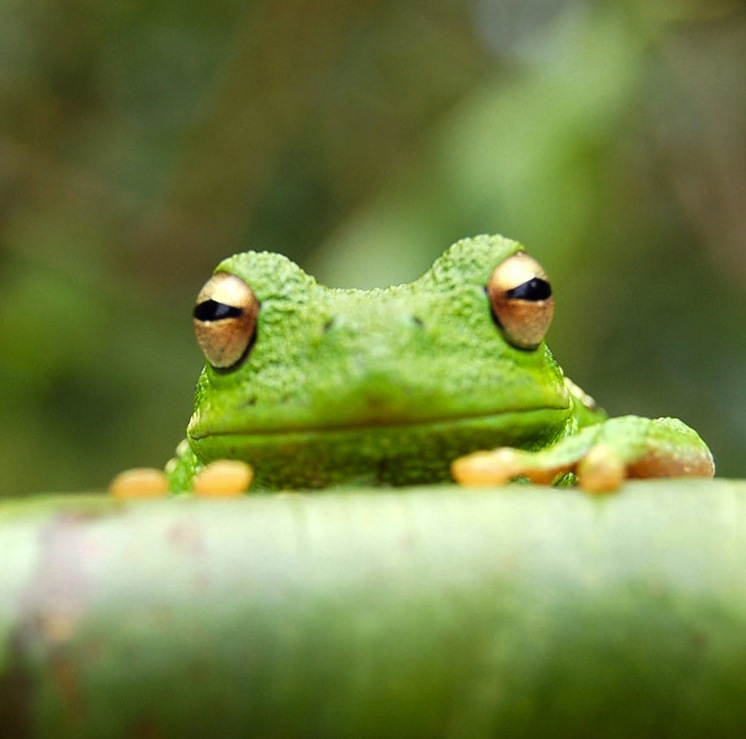
\includegraphics[width=0.25\textwidth]{frog.jpg}
\caption{\label{fig:frog2}This is a figure caption.}
\end{wrapfigure}

\lipsum[2-3]

\end{document}